\chapter{Implementation}
\label{cha:implementation}

The goal of this thesis is not only to come up with a concept that might work in practice: in order to prove the concept, this research consists out of the implementation of a working proof-of-concept. All source code of the proof-of-concept is released under the MIT licence, including the latex source code of this master thesis\footnote{\url{https://github.com/lightning-sprinkle}}.

\section{Universal automated payment solution}
The proof of concept that is developed is called Lightning Sprinkle. This name comes from two aspects of this system. Firstly, it uses the Lighting Network as a micropayment processor. Most systems related to the Lightning Network are referring so in their name. Secondly, sprinkle comes from the verb sprinkling, which is used in the fairy tale of Hansel and Gretel by the Brothers Grimm. In this story, Hansel and Gretel are walking away from home and sprinkling breadcrumbs along their path. Just like this, the sprinkle system leaves a trail of small payments along the browsing path.
\begin{figure}[h!]
  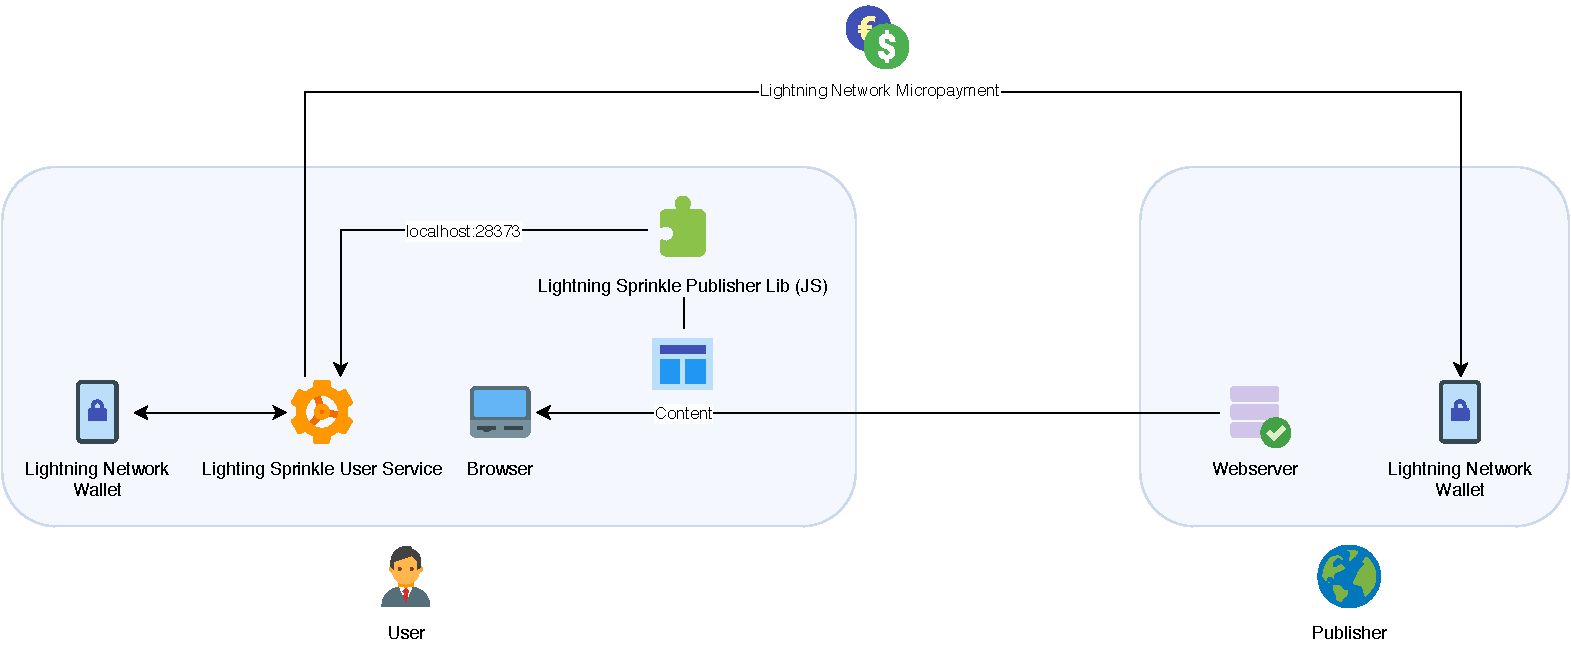
\includegraphics[width=\textwidth]{images/implementation.pdf}
  \caption{Schematic overview}
\end{figure}
In the remainder of this chapter, the following references are used:

\begin{description}
  \item[Lightning Sprinkle User Service] \hfill \\ A service that runs on the users' computer that handles the payments.
  \item[Lightning Sprinkle Publisher Lib] \hfill \\ A JavaScript library that is implemented by the publisher in order to request the payment.
\end{description} 

\subsection{Lightning Sprinkle Publisher Library}
According to the concept, as discussed in the part about WebRTC, there needs to be a method for the publisher to communicate with a system on the users' computer that handles the payment to the publisher. Usually, it is not easy to communicate with services that are running on the users' computer, because this might introduce security flaws as this exposes the computer to any script on any website that is visited. The standard way of interaction between the website and other software on the computer is using a browser extension. This, however, adds an extra step in the installation process. Therefore, other ways of interaction are researched.

\subsubsection{WebRTC}

WebRTC enables peer-to-peer connections between any website or server, which also includes connections between websites and services on one computer. The main idea is that the Publisher Library does some port scanning on the users' computer and connects to the User Service.

During the implementation, it turned out that it is impossible to create a webRTC connection between two instances directly. Compared to traditional TCP connections, it is not possible to connect to an arbitrary port without a proper handshake beforehand. The handshake and discovery process as implemented in the webRTC protocol is called signaling. Normally, this handshake is handled by a signaling server that functions as a handshake broker.

Unfortunately, introducing a central authority that handles the handshakes would disrupt the decental aspect of the entire system. Several alternatives are discussed, such as creating a decentralized network of signaling servers, however this would make the situation far more complex for such a small part of the entire ecosystem. Therefore, this approach is abandoned after a few experiments.

\subsubsection{postMessage()}
A different method of passing messages between different websites is the \textit{postMessage} functionality in JavaScript. This makes it possible to interact with different websites. In order to use the \textit{postMessage} method, there needs to be a link between both websites. Such a link only exists when one website is opened by another. This happens for example when website A opens website B in a new window or tab. The same link also exists when website B is loaded into an iFrame. 

Using this message system, it is possible for the Publisher Library to communicate with an instance of the User Service. The disadvantage of this approach is that it is limited to the web ecosystem: messages can only be transmitted to other websites, not to services that are running on the users' computer. 

On the basis of advancing insights, during experiments with the Lightning Network, it turned out that it is not feasible to create a system that runs completely inside the web ecosystem. Therefore, this approach is limited to the exploration phase and not implemented in the prototype.

\subsubsection{Localhost}
\label{sec:localhost}

The final approach to the problem of connecting from the Publisher Library to the User Service is using localhost. The idea stems from how the video conferencing tool Zoom connects to their software from an arbitrary website. The principle builds on the fact that it is possible to load content from websites that are hosted on another domain. This also includes localhost.

In practice, any website can connect to any other domain. Examples of applications can be found in abundance in web tracking. For example, if a user visits a website that uses third party tracking, a request is made to the third party from the users' computer to send data, such as tracking cookies, to the ad network. 

This implementation aims to enable the Publisher Library to connect to the User Service on the local machine in order to request an automated payment. The User Service includes a web server that can be accessed by the Publisher Library. 

The ability to create requests to different domains introduces plenty of security issues. It might leak data that is only intended for the user on other domains or even trigger an action on another website. This is known as Cross Site Scripting (XSS) vulnerabilities. Therefore, browsers have taken security measures in order to prevent these undesired side effects.

Firstly, as a website, it is possible to configure the Cross-Origin Resource Sharing (CORS). This parameter can limit the amount of websites that are allowed to send a request to them. Secondly, so-called mixed content is not allowed. This means that if the website runs on HTTPS and initiates a request to a third party that is on HTTP, the request is blocked by the browser. Thirdly, Chrome is actively blocking any requests to localhost, as this might expose services that are running on the local machine.

The first security measure can be circumvented easily by setting \\\texttt{Access-Control-Allow-Origin:*}, which means that any publisher using the Publisher Library is able to connect to the User Service. 

The second measure is harder to circumvent. These days, every self-respecting website uses HTTPS, which makes it impossible to not support the Publisher Library on HTTPS websites. There are a couple of workarounds to make it possible to support HTTPS enabled publishers to connect to localhost:

%twijfel over deze dubbele punt. En daarnaast: de eerste zin hieronder is nogal abrupt: ineens is het probleem opgelost. Twijfel of je daar iets meer woorden aan vuil moet maken.
 
Firstly, the User Service can support HTTPS. However, in order to support HTTPS, there needs to be a certificate that is used to encrypt the traffic to localhost. Such a certificate can only be issued if a domain name is used. With localhost, this is not the case. So, the only option is to generate a self-signed certificate. Self-signed certificates, however, are not trusted by browsers, so requests are still blocked. To support this self-signed certificate, the user needs to make an exception in the browser for this particular certificate. This method is not very user-friendly and violates the zeroconf principle, which makes it suboptimal.

Secondly, an exception is made by the browser for media content that is being loaded from external resources. The standard way of performing requests to another website from Java\-Script is using an \texttt{XMLHttpRequest}, but these requests are facing limitations like the one on self-signed certificates. On the other hand, when a website just embeds an image from another website, there are very little limitations. Fortunately, it is possible to load an image in a programmed way and transfer data using this image.

The implementation of this is quite simple: the Publisher Library loads an image that is located on localhost, for example: \texttt{http://localhost:28373/status}. Then the User Service receives the request and is able to answer with an image. The content cannot be extracted easily in the Publisher Library, but metadata like the dimensions of the image are easy to read. Using this approach, a two-way communication is possible between the Publisher Library and the User Service. The User Service responds to the request by sending an image with a particular dimension. In this case, for example, responding with an image that has a width of 2, means that the system is running and the publisher is approved.


\lstset{language=JavaScript}
\lstset{frame=lines}
\lstset{caption={Communication with Lightning Sprinkle User Service}}
\lstset{label={lst:code_direct}}
\lstset{basicstyle=\footnotesize}
\begin{lstlisting}
/**
* Check if lightningSprinkle is running and if this domain 
* has been approved by the user.
* @return {Promise:String} status
*/
function getStatus() {
  return new Promise((resolve, reject) => {
    let statusImage = new Image();
    statusImage.referrerPolicy = "unsafe-url"
    statusImage.src = 'http://localhost:28373/status?' + Math.random()
    statusImage.decode()
    .then(() => {
      if (statusImage.width === 1) {
        resolve('new')
      } else if (statusImage.width === 2) {
        resolve('accepted')
      } else if (statusImage.width === 3) {
        resolve('rejected')
      }
    })
    .catch((encodingError) => {
      resolve('offline')
    })
  })
}
\end{lstlisting}

\subsubsection{Asking for permission}
As stated in Chapter \ref{cha:conceptanddesign}, the system determines the credibility of a website by checking the type of certificate the publisher has. If this certificate is based on organization validation (OV), the system pays to the publisher automatically. For smaller publishers, who cannot afford such a certificate, the Publisher Library can request permission to get paid. 

The system that asks for permission also relies on the web ecosystem. The Publisher Library checks if this publisher is permitted. If this is not the case, a pop-up window is opened which opens a web page that is hosted on localhost by the User Service. The User Service is able to find out which publisher made the request by reading the referral header. The user is able to accept the request, which adds the domain name to the whitelist. In the future, this publisher is also able to request automated payments.

\begin{figure}[h!]
  \setlength{\fboxsep}{0pt}%
  \fbox{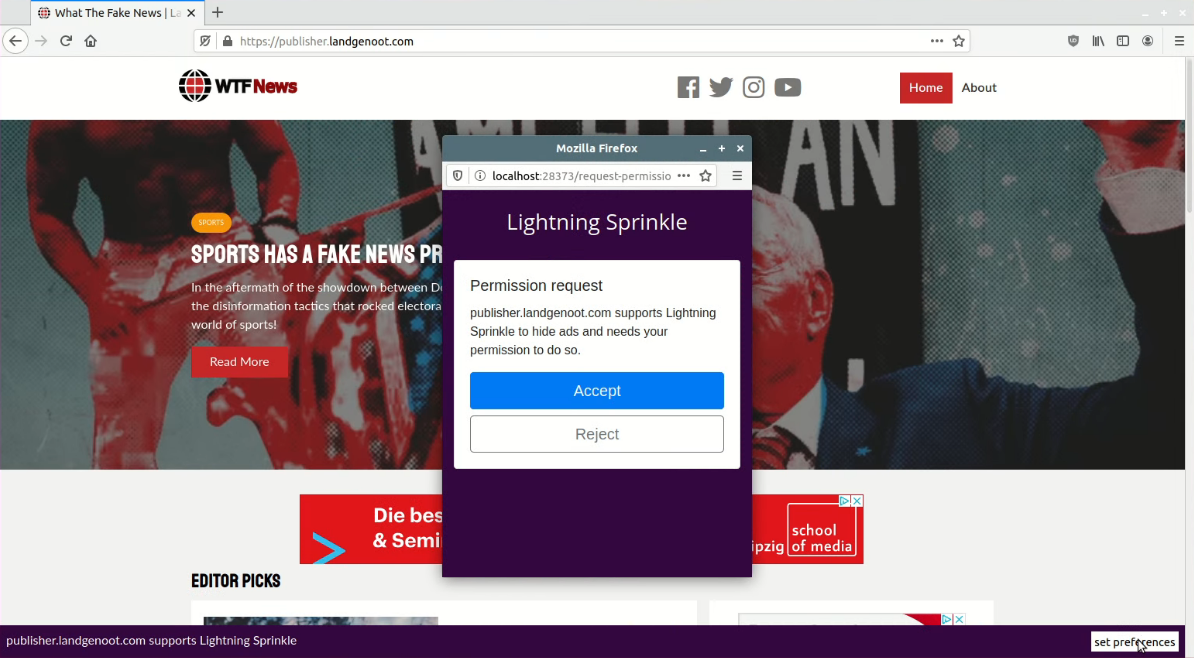
\includegraphics[width=\textwidth-2px]{images/popup.png}}
  \caption{Pop-up that asks for permission}
\end{figure}

\subsection{Lightning Network}
\label{sec:lightningnetwork}

Now there is an ecosystem that enables publishers to communicate with a service that runs outside the browser. This service, somehow, needs to make a micropayment. As discussed in Chapter \ref{cha:relatedwork}, existing payment service providers are not suitable since they violate the decentralized principle. Therefore, the landscape of cryptocurrencies that are suitable for micropayments is researched. It turned out that the Lightning Network is the most promising solution, as it relies on the cryptocurrency with the largest market capacity and is still able to process instant payments with minimal fees. The principle of the Lightning Network is already explained in Chapter \ref{cha:conceptanddesign}. This section explains what challenges were faced during the implementation of the proof-of-concept.

The Lightning Network is not a single implementation. The creators of the Lightning Network decided to create a Request For Comments (RFC) instead. This RFC describes how the network should function and by what rules. Several other parties are implementing clients that follow this standard. However, because of the current work-in-progress state of the system, there are small differences between the clients and even between different versions of clients. 

In order to run a Lightning Node, which is a client that is part of the network, an application with multiple components is needed. 

Firstly, there is a normal client, in order to communicate with the network and perform transactions on the blockchain. This client also takes care of the private keys that are needed to sign any transaction.

Secondly, there needs to be a Lightning Network Node. This client handles all the communication with the Lightning Network, and also interacts with the client in order to open or close channels. 

Thirdly, since all the transactions that occur over the Lightning Network are easy to follow, there needs to be some form of obfuscation. The Onion Router (TOR) \cite{mccoy2008shining} is used to anonymize the interaction with the network. Otherwise, it will be easy to link an IP address to a Lightning transaction.

%En waarom is dat een probleem?

\begin{figure}[h!]
  \setlength{\fboxsep}{0pt}%
  \center
  \fbox{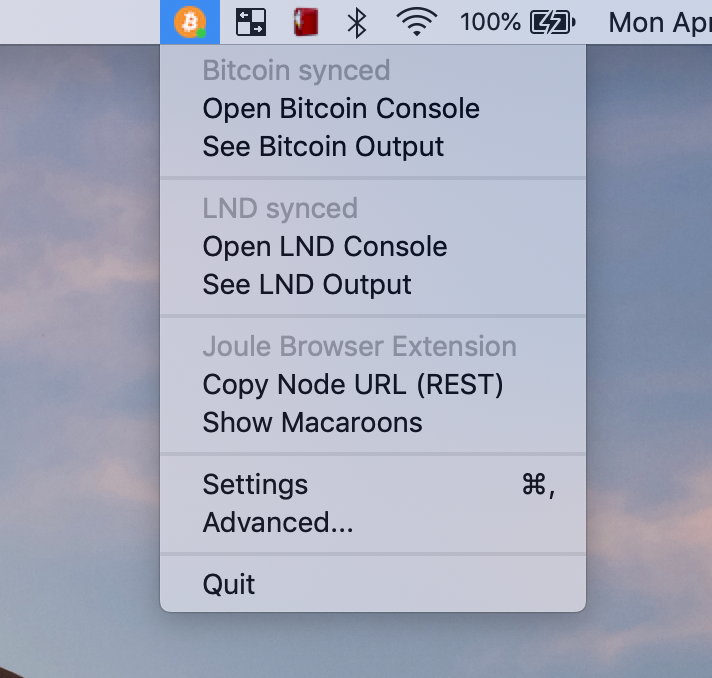
\includegraphics[width=15em]{images/node-launcher.png}}
  \caption{The node-launcher application}
\end{figure}

The node-launcher can be described as package bundle with all the components listed above, written in Python. It takes care that all the components are configured correctly and are up and running. It also features a tray application that shows the status of the application. In the first phase, this application is adopted as a lighting network solution as this application is easily modifiable.

When the node-launcher is running, there is no GUI to interact with the Lightning Network node. It is up to the user to install a front-end that interacts with the Lightning Node. Examples of these front-ends are the Zap wallet\footnote{\url{https://github.com/LN-Zap/lnd}} or the Joule Browser Extension\footnote{\url{https://github.com/joule-labs/joule-extension}}. For this thesis, however, there is no need for a front-end, as the Lightning Sprinkle User Service is able to interact with the Lightning Node directly. 

The design of a Lightning Network transaction is based on a one-time invoice structure. The receiver of the payment needs to create such an invoice first, which will be transmitted in the form of an encoded string or QR-code. This invoice contains details like the amount, payee public key, routing hints and an expiration date. The payor opens this invoice in the lighting network node application, and after that is able to submit the payment.

Due to this structure, it is very hard to make spontaneous payments. When selling products online, there is no objection against such a structure, but for other things than goods and services, it is not ideal. This is for example the case with donations. Currently, there are services that offer to create a Lightning Network donate button that generates a new invoice every time it is accessed. Under the hood, these services are connecting to the Lightning Network node of the payee and requesting a new invoice every time. For the purpose of this thesis, this is far from ideal, because that means that while visiting any website, multiple other requests are needed in order to exchange the invoice. 

\subsubsection{Keysend}
\label{sec:keysend}

The Lightning Network is currently still in an experimental phase and under active development. During the implementation phase of this thesis, the team behind the lnd client, which is an implementation of the Lightning Network, explored a way to circumvent the invoice structure\footnote{\url{https://github.com/lightningnetwork/lnd/pull/3795}}. This feature is not yet part of the official Lightning Network specification, and therefore also not (yet) widely supported. During the implementation phase of this proof-of-concept, it was only possible to experiment with this circumvention, by using the latest beta version of the lnd client. 

The implementation only exists in the latest \texttt{lncli} client. This command line tool connects to the \texttt{lnd} node and is able to interact with it. For example, it can create invoices. If both the payor and the payee are using the latest version of \texttt{lnd} and it is started with the \texttt{--accept-key-send} flag, it is possible to send spontaneous payments using the \texttt{--keysend} flag. It does not matter what configuration, client or version of the Lightning Network the nodes in between are using. 

Unfortunately, the Lighting Sprinkle User Service needs to connect to the \texttt{lnd} node directly and does not make use of the \texttt{lncli}. Therefore, it is not a matter of setting the \texttt{--keysend} flag and a deeper understanding of the workaround is needed.

The workaround, however, is not as straight forwarded as it seems to be. Normally, the invoice contains a hash of the preimage. The preimage is a cryptographically random bytearray with size 32, that is needed in order to redeem a locked payment. If there is no invoice, we cannot exchange this secret with the payor. To circumvent this issue, \texttt{lnd} makes use of a custom record as part of the payment.

\texttt{KeySendRecord uint64 = 5482373484}

The custom record with this ID, contains a preimage that is generated by the payor. Only the payee is able to read these custom records and is therefore also able to redeem the payment. The rest of the payment occurs in the standard way.
\lstset{language=Python}
\lstset{frame=lines}
\lstset{caption={Constructing a keysend SendRequest}}
\lstset{label={lst:code_direct}}
\lstset{basicstyle=\footnotesize}
\begin{lstlisting}
def keysend_money(dest, amt):
  """ 
  Transfer money using the experimental keysend method
  """
  # Generate preimage by generating cryptographic safe random bytes
  preimage = secrets.token_bytes(32) 
  payment_hash = hashlib.sha256(preimage).digest()
  # Set the preimage as a custom record in order 
  # to use the experimental keysend method
  dest_custom_records = {5482373484: preimage}

  request = ln.SendRequest(
    dest_string=dest,
    amt=amt,
    final_cltv_delta=40,
    payment_hash=payment_hash,
    dest_custom_records=dest_custom_records
  )
  
  return stub.SendPaymentSync(request, metadata=[('macaroon', macaroon)])

\end{lstlisting}

Interestingly, the custom record functionality is also implemented quite recently. One of the use cases for these custom records are to exchange chat messages over the Lightning Network (whatsat), so that it acts like a decentralized messaging service. Another use case is that the payment contains data about an online webshop order, so that it becomes possible to buy products or services atomically.


\subsection{Lightning Sprinkle User Service}

The User Service is the component that handles all the requests from the publishers that have implemented the Publisher Library. In order to do so, an application in Python is built on the Flask framework. This framework makes it easy to create an application in Python that also provides an API.

This application consists out of six modules:
\begin{enumerate}
  \item server
  \item reward
  \item status image
  \item lnd
  \item dns
  \item cert 
\end{enumerate}

Firstly, the server part functions as a web server. There are three different API-endpoints: status, request-permission and request-payment. The status endpoint returns whether the origin domain of the request is allowed to request payments. The request-permission endpoint is used to add the origin domain to the whitelist. Lastly, the request-payment endpoint is used to request and execute the automated payment.

Secondly, the reward module keeps track of the budget. Based on a maximal hourly reward, the fee is calculated and used in the micropayments.


\lstset{language=Python}
\lstset{frame=lines}
\lstset{caption={Reward system}}
\lstset{label={lst:code_direct}}
\lstset{basicstyle=\footnotesize}
\begin{lstlisting}
  import threading
  import config
  
  bucket = config.max_hourly_reward
  
  def fill_bucket():
    """
    Make sure the bucket stays filled by adding the 1/60 of the max_hourly_reward
    every minute.
    """
    global bucket
    threading.Timer(60, fill_bucket).start()
    bucket = min(bucket + (config.max_hourly_reward / 60), config.max_hourly_reward)
  
  def get_current_reward():
    """
    Calculate the current reward based on the level of the bucket
    """
    global bucket
    reward = int(bucket * 0.25)
    bucket = bucket - reward
    return reward
\end{lstlisting}

Thirdly, the status image module generates an image with given dimensions. This image is used as a workaround in order to support two-way communication, as described in Section \ref{sec:localhost}.

Fourthly, the lnd module handles the communication with the Lightning Network node. This communication is based on gRPC. It provides a function that is able to send a payment to an address immediately using the keysend method. The keysend method is described in more detail in Section \ref{sec:keysend}. In order to authenticate at the lnd service, macaroons are used. Macaroons are comparable to cookies and contain authentication data. They are implemented in such a way that different types of macaroon provide different levels of privilege. 

Fifthly, the dns module takes care of the extraction of the DNS entries. As described in Chapter \ref{cha:conceptanddesign}, the payment needs to have a destination. Storing the public key of the destination in JavaScript, introduces potential vulnerabilities as user generated content is able to alter JavaScript. Therefore, the service relies on TXT-records that are stored at the DNS server. In this way it is guaranteed that the recipient of the payment also controls the DNS records of the domain. This module implements a DNS resolver and looks for a TXT-record that contains a public key according to the following format:

\texttt{lnd-pubkey=027d2456f6d4aaf27873b68b7717b...}

Lastly, the cert module is able to check the credibility of the domain name by looking up the type of certificate that is used. As described in Chapter \ref{cha:conceptanddesign}, the presence of an OV or EV certificate indicates enough credibility to automate the payment immediately. 

SSL certificates are structured according to the X509 format. These certificates contain basic info, like the certificate authority and the organization. As the X509 format is designed in 1988 \cite{biddle2009browser}, long before certificates were used for HTTPS, it does not have any option to store the type of certificate directly. In order to differentiate between DV, OV and EV certificates, a certificate extension called \textit{CertificatePolicies} is used. The following policies with corresponding object IDs are used for the different types of certificates:

\begin{enumerate}[leftmargin=8em]
  \item[2.23.140.1.2.1] Domain Validation
  \item[2.23.140.1.2.2] Organization Validation
  \item[2.23.140.1.1] Extended Validation
\end{enumerate}

By extracting these \textit{CertificatePolicies}, it is possible to determine the type of certificate that a particular domain name uses. 


\lstset{language=Python}
\lstset{frame=lines}
\lstset{caption={Check if a hostname is an organization}}
\lstset{label={lst:code_direct}}
\lstset{basicstyle=\footnotesize}
\begin{lstlisting}
import ssl
from cryptography import x509
from cryptography.hazmat.backends import default_backend

def isOrganization(hostname):
  """
  Function looks up the SSL certificate for the domain, and checks if 
  it is an OV or EV certificate by reading the following CertificatePolicies
  2.23.140.1.2.2: Organization Validation
  2.23.140.1.1: Extended Validation 
  """

  # Create a real connection in order to support SNI (server name indication)
  conn = ssl.create_connection((hostname, 443))
  context = ssl.SSLContext(ssl.PROTOCOL_SSLv23)
  sock = context.wrap_socket(conn, server_hostname=hostname)
  cert_pem = ssl.DER_cert_to_PEM_cert(sock.getpeercert(True))
  cert = x509.load_pem_x509_certificate(cert_pem.encode(), default_backend())
  
  # Find the certificate type
  for policy in cert.extensions.get_extension_for_class(x509.CertificatePolicies).value:
    oid = policy.policy_identifier.dotted_string
    if oid == '2.23.140.1.2.2' or oid == '2.23.140.1.1':
      return True

  return False
\end{lstlisting}

\subsection{Electron tray application and Neutrino}
\label{sec:electron}
The first proof-of-concept, as described in Section \ref{sec:lightningnetwork}, uses the normal full \texttt{btcd} daemon. The disadvantage of this method, is that the entire blockchain needs to be downloaded. As of 2020, this is over 300GB and takes over 24 hours on an average DSL Internet connection. 

However, there are also so-called light wallets available, which do not require the entire blockchain to be downloaded. They rely on other nodes and only download the blocks after a certain block number. In order to only download transactions that are relevant for the user, bloom filters are used. Bloom filters make sure that a part of all transactions is downloaded that at least include the transactions of the user. However, because not only the transactions of the user are downloaded, but also a couple of transactions of several other users, the privacy of the user is preserved.

The \texttt{lightning-app}\footnote{\url{https://github.com/lightninglabs/lightning-app}} uses the \texttt{neutrino}\footnote{\url{https://github.com/lightninglabs/neutrino}} light wallet, which makes it much less of a hassle to set up a Lightning Node. This \texttt{lightning-app} does not require to download the entire blockchain. Moreover, the \texttt{lightning-app} also features an autopilot mode, where it automatically opens Lightning channels, so that the user is able to spend money. This approach makes the proof-of-concept of this thesis much more viable. 

In the second phase of the implementation, two new aspects of this system are introduced: the transition to JavaScript/Electron and the use of the Neutrino Bitcoin light wallet.

In electron, it is also possible to create a tray application, so that the application keeps running when closed. 


\begin{figure}[h!]
  \setlength{\fboxsep}{0pt}%
  \center
  \fbox{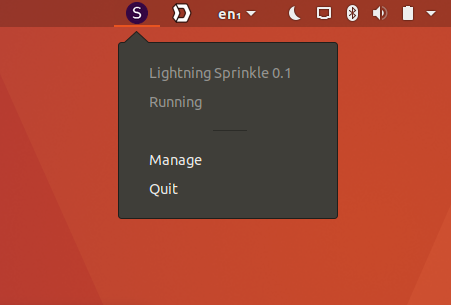
\includegraphics[width=20em]{images/electron-tray.png}}
  \caption{The Lightning Sprinkle Tray Application}
\end{figure}

Unfortunately, the translation to JavaScript/Electron took more time than expected. As this thesis is only about developing a proof-of-concept, the development of this alternative implementation is not continued.

\subsection{Example website with Google AdSense}
\label{sec:examplesite}

\begin{figure}[h!]
  \setlength{\fboxsep}{0pt}%
  \fbox{
\includegraphics[width=\textwidth-2px]{images/example-website.png}}
  \caption{Example website with ads that implements the Lightning Sprinkle Publisher Library}
\end{figure}

In order to demonstrate the project, a small static website is set up using an open source template. This demo website shows how a publisher can implement the Lightning Sprinkle Publisher Library. 

To make the example as realistic as possible, the Google AdSense program is added, so that Google is able to serve real advertisements on the demo website. 

One problem with such a third party supplier of advertisements like Google, is that normally there is no toggle to disable the advertisements other than not loading the JavaScript library of the advertisement network. Unofficially, however, it is possible to disable advertisements in the same way they are blocked by an Ad Blocker: by removing certain objects from the Document Object Model (DOM). For Google AdSense, this is done by the following simple JavaScript line:


\lstset{language=JavaScript}
\lstset{frame=lines}
\lstset{caption={Disabling Google AdSense advertisements}}
\lstset{label={lst:code_direct}}
\lstset{basicstyle=\footnotesize}
\begin{lstlisting}
  $('.adsbygoogle').remove()
\end{lstlisting}

Using this unofficial method, it becomes possible to let the user decide if he or she either wants to see advertisements or to allow the publisher to request automated payments instead.

The purple bar on the bottom of the example website is added by the Lightning Sprinkle Publisher Library. The button at the bottom can be used to add the publisher to the whitelist.
